You probably learned about linked lists in \cstwo; however, we will provide a refresher.

A \textit{linked list} is a linear collection of data.
Like an array, each element (or \textit{node}) has a particular position in the list, and when you iterate over the list, you always access the elements in the same order every time (unless you change or re-order the elements).

In an array, the elements are contiguous in memory, and you can access a specific element by indexing the array (or, equivalently, performing pointer arithmetic).
In a linked list, however, the nodes can be in arbitrary locations in memory, and the nodes are connected by references (in C, pointers).
You can access a specific element only by following pointers from one node to the next until you reach the desired node.


\subsection{Singly-Linked List} \label{subsec:singlylinkedlist}

The simplest linked list is a \textit{singly-linked list}.
A node consists of a \textit{payload} (the data that we care about) and a reference to the \textit{next} node;
see Figure~\ref{fig:singly-linked-list}.

\begin{figure}[h]
    \centering
    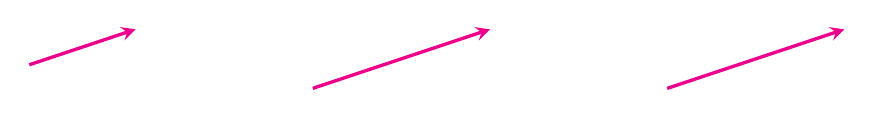
\begin{tikzpicture}[x=1.5mm, y=1.5mm]
        \draw[-stealth,very thick,magenta](-19,-3) -- (-10,0);
        \sllnode{0}{0}{0}
        \draw[-stealth,very thick,magenta](5,-5) -- (20,0);
        \sllnode{30}{0}{0}
        \draw[-stealth,very thick,magenta](35,-5) -- (50,0);
    \end{tikzpicture}
    \caption{Nodes in a singly-linked list consist of the payload data and a reference that points to the next node.}\label{fig:singly-linked-list}
\end{figure}

A linked list's greatest advantage over an array is that inserting and removing a node at an arbitrary location takes constant time, whereas inserting an element into an array (assuming there is sufficient memory allocated for the array) or removing an element from an array requires moving all the elements that follow the element's index.
Inserting a new node, $C$, between adjacent nodes $A$ and $B$ (where $B = A.next$) requires connecting $C.next$ to $B$ and re-assigning $A.next$ to $C$;
see Figure~\ref{fig:sll-insertion}.

\begin{figure}[h]
    \centering
    \begin{tikzpicture}[x=1.5mm, y=1.5mm]
        \draw[-stealth,very thick,magenta](-19,-3) -- (-10,0);
        \sllnode{0}{0}{0}
        \draw[-stealth,very thick,magenta](5,-5) -- (13,-5) -- (13,-12.5) -- (0,-12.5) -- (0,-25) -- (5,-25);
        \sllnode{15}{-25}{0}
        \draw[-stealth,very thick,magenta](20,-30) -- (30,-30) -- (30,-12.5) -- (17,-12.5) -- (17,0) -- (20,0);
        \sllnode{30}{0}{0}
        \draw[-stealth,very thick,magenta](35,-5) -- (50,0);
    \end{tikzpicture}
    \caption{Inserting a new node into a singly-linked list only requires assignments to the affected \textit{next} pointers.}\label{fig:sll-insertion}
\end{figure}

As with an array, you do need to maintain a variable that points to the list.
Conventionally, this is a reference to the \textit{head} of the list.
(Note that if a new node is inserted before the current head node, then the new node becomes the head of the list, and your \lstinline{head} variable would need to be updated.)
It is not uncommon to also maintain a reference to the \textit{tail} of the list.

%\subsection{Circular Linked List} \label{subsec:circularlinkedlist}
%
%A \textit{circular linked list} is a linked list in which the tail's \textit{next} field points to the head of the list.
%In essence, a circular linked list has no head (because every node is some node's \textit{next}), and has no tail (because every node's \textit{next} is non-NULL);
%see Figure~\ref{fig:circular-linked-list}.
%
%\begin{figure}[h]
%    \centering
%    \begin{tikzpicture}[x=1.5mm, y=1.5mm]
%        \sllnode{0}{30}{0}
%        \draw[-stealth,very thick,magenta,rotate=0](5,25) -- (25.5,18.8);
%        \sllnode{0}{30}{-72}
%        \draw[-stealth,very thick,magenta,rotate=-72](5,25) -- (25.5,18.8);
%        \sllnode{0}{30}{-144}
%        \draw[-stealth,very thick,magenta,rotate=-144](5,25) -- (25.5,18.8);
%        \sllnode{0}{30}{144}
%        \draw[-stealth,very thick,magenta,rotate=144](5,25) -- (25.5,18.8);
%        \sllnode{0}{30}{72}
%        \draw[-stealth,very thick,magenta,rotate=72](5,25) -- (25.5,18.8);
%    \end{tikzpicture}
%    \caption{A circular linked list does not have a well-defined head and tail.}\label{fig:circular-linked-list}
%\end{figure}
%
%You still need to maintain a variable that points to \textit{some} node in the list.


\subsection{Doubly-Linked List} \label{subsec:doublylinkedlist}

A \textit{doubly-linked list} is a linked list with the property that each node maintains a link not only to the \lstinline{next} node but also a link to the \lstinline{previous} node.
In C, these links are pointers.

\begin{figure}[h]
    \centering
    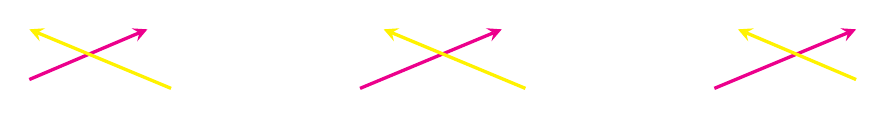
\begin{tikzpicture}[x=1.5mm, y=1.5mm]
        \draw[-stealth,very thick,magenta](-20,-4.25) -- (-10,0);
        \draw[stealth-,very thick,yellow](-20,0) -- (-8,-5);
        \dllnode{0}{0}{0}
        \draw[-stealth,very thick,magenta](8,-5) -- (20,0);
        \draw[stealth-,very thick,yellow](10,0) -- (22,-5);
        \dllnode{30}{0}{0}
        \draw[-stealth,very thick,magenta](38,-5) -- (50,0);
        \draw[stealth-,very thick,yellow](40,0) -- (50,-4.25);
    \end{tikzpicture}
    \caption{Nodes in a doubly-linked list consist of the payload data and references that point to the previous and next nodes.}\label{fig:doubly-linked-list}
\end{figure}

Inserting new node, $C$, between adjacent nodes $A$ and $B$ (where $B = A.next$ and $A = B.previous$) requires connecting $C.previous$ to $A$ and $C.next$ to $B$, and re-assigning $A.next$ to $C$ and $B.previous$ to $C$.



\subsection{Equivalent Java Code} \label{subsec:equivalentjava}

In Java, you probably wouldn't implement your own linked list;
instead, you would use \lstinline{java.util.LinkedList}, which has been available since J2SE~1.2.
%(ignoring for the moment that Java's standard library doesn't have a circular linked list).
A list of \lstinline{WordEntry} objects would be created with:
\begin{lstlisting}[numbers=none]
    List<WordEntry> wordEntries = new LinkedList<>;
\end{lstlisting}

C doesn't have a built-in linked list data type, so you will need to design one.
Let us consider what a custom linked list would look like in Java.

\begin{lstlisting}[mathescape=true]
public class WordEntry {
    private final String word;          $\label{code:javaWord}$
    private int occurrences;            $\label{code:javaOccurrences}$ $\lstsetnumber{\ldots}$
    ...$\lstresetnumber\setcounter{lstnumber}{53}$
}
\end{lstlisting}

\begin{lstlisting}[firstnumber=100, mathescape=true]
public class Node {
    private final WordEntry wordEntry;  $\label{code:javaPayload}$
    private Node next;                  $\label{code:javaNext}$
    private Node previous;              $\label{code:javaPrevious}$

    public Node(WordEntry wordEntry) {$\lstsetnumber{\ldots}$
        ...$\lstresetnumber\setcounter{lstnumber}{111}$
    }
    $\lstsetnumber{\ldots}$
    ...$\lstresetnumber\setcounter{lstnumber}{203}$
}
\end{lstlisting}

\begin{lstlisting}[firstnumber=309, mathescape=true]
public class MyLinkedList {
    private Node head;
    private Note tail;
    private Node current;

    public MyLinkedList() {$\lstsetnumber{\ldots}$
        ...$\lstresetnumber\setcounter{lstnumber}{320}$
    }

    public void insert(WordEntry wordEntry) {
        Node node = new Node(wordEntry){$\lstsetnumber{\ldots}$
        ...$\lstresetnumber\setcounter{lstnumber}{329}$
    }
    $\lstsetnumber{\ldots}$
    ...$\lstresetnumber\setcounter{lstnumber}{417}$
}
\end{lstlisting}

Creating and inserting a new word entry would look something like this:

\begin{lstlisting}[firstnumber=450, mathescape=true]
    WordEntry wordEntry = new WordEntry("eggplant");    $\label{code:newWordEntry}$
    list.resetIterator();
    while (...) list.iterateForward(); // determine where new node goes
    list.insert(wordEntry);                             $\label{code:javaInsert}$
\end{lstlisting}

Recall that in Java, all variables except primitive types (such as \lstinline{occurrences} on line~\ref{code:javaOccurrences}) are references.
This means that the \lstinline{next} field on line~\ref{code:javaNext} is a reference to another Node, just as we described in Section~\ref{subsec:singlylinkedlist}.
The payload is the \lstinline{wordEntry}.

\subsubsection{C Implementation} \label{subsubsec:cImplementation}

In \textit{linked-list.h}, you'll see a \lstinline{struct}s with the same fields as our Java example:

\lstinputlisting[linerange=41-45, firstnumber=41]{../starter-code/linked_list.h}

\lstinputlisting[linerange=56-60, firstnumber=56]{../starter-code/linked_list.h}

In \textit{linked\_list.c}, you'll also see the \function{create_node()} and \function{create_list()} functions:

\lstinputlisting[linerange=29-33, firstnumber=29]{../starter-code/linked_list.c}

\lstinputlisting[linerange=61-66, firstnumber=61]{../starter-code/linked_list.c}

As you can see, they allocate space for a new node or a new list handle using \function{malloc()}.
The code that you will need to add to \function{create_node()} will copy the \lstinline{word_entry} argument into the \lstinline{word_entry} field.
Since we don't yet know where this node will go, set the node's \lstinline{next} and \lstinline{previous} pointers to point to NULL\@.
The code that you will need to add to \function{create_list()} is even simpler: a newly-created list is empty, and so it has no head, no tail, and no current node.


\subsection{A Visualization of the Data Types}

\subsubsection{word\_entry\_t}

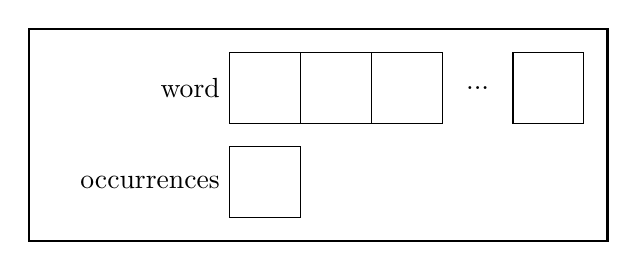
\begin{tikzpicture}[x=1.5mm, y=1.5mm]
    \draw[thick] (0,0) rectangle (49,18);
    \draw (17,16) rectangle ++(6,-6) +(-6,3) node[anchor=east] {word};
    \draw (23,16) rectangle ++(6,-6) rectangle ++(6,6) +(3,-3) node {...};
    \draw (41,16) rectangle ++(6,-6);
    \draw (17,8) rectangle ++(6,-6) +(-6,3) node[anchor=east] {occurrences};
\end{tikzpicture}

\subsubsection{node\_t}

\begin{tikzpicture}[x=1.5mm, y=1.5mm]
    \draw[thick] (0,0) rectangle (25,26);
    \draw (17,24) rectangle ++(6,-6) +(-6,3) node[anchor=east] {word\_entry};
    \draw (17,16) rectangle ++(6,-6) +(-6,3) node[anchor=east] {next};
    \draw (17,8) rectangle ++(6,-6) +(-6,3) node[anchor=east] {previous};

    \draw (40,24) rectangle ++(+10,-6) +(-5,3) node (word) {\tiny{word\_entry\_t}};
    \draw[Circle-Stealth,very thick] (20,21) -- (word.west);
    \draw (40,16) rectangle ++(6,-6) +(-3,3) node (next) {\tiny{node\_t}};
    \draw[Circle-Stealth,very thick] (20,13) -- (next.west);
    \draw (40,8) rectangle ++(6,-6) +(-3,3) node (previous) {\tiny{node\_t}};
    \draw[Circle-Stealth,very thick] (20,5) -- (previous.west);
\end{tikzpicture}

\subsubsection{list\_t as an array-backed list}

\begin{tikzpicture}[x=1.5mm, y=1.5mm]
    \draw[thick] (0,0) rectangle (25,34);
    \draw (17,32) rectangle ++(6,-6) +(-6,3) node[anchor=east] {array};
    \draw (17,24) rectangle ++(6,-6) +(-6,3) node[anchor=east] {length};
    \draw (17,16) rectangle ++(6,-6) +(-6,3) node[anchor=east] {allocation};
    \draw (17,8) rectangle ++(6,-6) +(-6,3) node[anchor=east] {index};

    \draw[Circle-Stealth,very thick] (20,29) -- (40,21);
    \draw (40,24) rectangle ++(6,-6) rectangle ++(6,6) rectangle ++(6,-6) ++(6,0) rectangle ++(6,6) +(-9,-3) node {...};
    \draw (70,24) rectangle ++(6,-6) ++(-3,3) node {X} ++(3,-3) rectangle ++(6,6) ++(-3,-3) node {X} ++(9,-3) rectangle ++(6,6) ++(-3,-3) node {X} +(-6,0) node {...};
    \draw[thin] (40,26) -- ++(0,8) ++(30,-8) -- ++(0,3.5) ++(24,-3.5) -- ++(0,8);
    \draw[<-, thin] (40,28) -- ++(11,0) node[anchor=west] {\footnotesize{length}};
    \draw[->, thin] (40,28) ++(19,0) -- ++(11,0);
    \draw[<-, thin] (40,32) -- ++(21,0) node[anchor=west] {\footnotesize{allocation}};
    \draw[->, thin] (40,32) ++(33,0) -- ++(21,0);

    \draw[Circle-Stealth,very thick] (43,21) -- (38,12);
    \draw (38,12) ++(-5,0) rectangle ++(+10,-6) +(-5,3) node {\tiny{word\_entry\_t}};
    \draw[Circle-Stealth,very thick] (49,21) -- (46,2);
    \draw (46,2) ++(-5,0) rectangle ++(+10,-6) +(-5,3) node {\tiny{word\_entry\_t}};
    \draw[Circle-Stealth,very thick] (55,21) -- (59,15);
    \draw (59,15) ++(-5,0) rectangle ++(+10,-6) +(-5,3) node {\tiny{word\_entry\_t}};
    \draw[Circle-Stealth,very thick] (67,21) -- (80,7);
    \draw (80,7) ++(-5,0) rectangle ++(+10,-6) +(-5,3) node {\tiny{word\_entry\_t}};
\end{tikzpicture}

\subsubsection{list\_t as a linked list}

\begin{tikzpicture}[x=1.5mm, y=1.5mm]
    \draw[thick] (0,0) rectangle (25,26);
    \draw (17,24) rectangle ++(6,-6) +(-6,3) node[anchor=east] {head};
    \draw (17,16) rectangle ++(6,-6) +(-6,3) node[anchor=east] {tail};
    \draw (17,8) rectangle ++(6,-6) +(-6,3) node[anchor=east] {current\_node};

    \draw (38,28) rectangle ++(6,-6) +(-3,3) node (head) {\tiny{node\_t}};
    \draw[Circle-Stealth,very thick] (20,21) -- (head.west);
    \draw (38,16) rectangle ++(6,-6) +(-3,3) node (tail) {\tiny{node\_t}};
    \draw[Circle-Stealth,very thick] (20,13) -- (tail.west);
    \draw (86,4) rectangle ++(6,-6) +(-3,3) node (current) {\tiny{node\_t}};
    \draw[Circle-Stealth,very thick] (20,5) -- (current.west);

    \draw (38,28)
        ++(12,0) rectangle ++(6,-6) ++(-3,3) node (node1) {\tiny{node\_t}}
        ++(9,3) rectangle ++(6,-6) ++(-3,3) node (node2) {\tiny{node\_t}}
        ++(9,3) rectangle ++(6,-6) ++(-3,3) node (node3) {\tiny{node\_t}}
        ++(9,3) rectangle ++(6,-6) ++(-3,3) node (node4) {\tiny{node\_t}}
        ++(9,3) rectangle ++(6,-6) ++(-3,3) node (node5) {\tiny{node\_t}}
        ++(-3,-9) rectangle ++(6,-6) ++(-3,3) node (node6) {\tiny{node\_t}}
        ++(-3,-9) rectangle ++(6,-6) ++(-3,3) node (node7) {\tiny{node\_t}}
        ++(-15,15) rectangle ++(6,-6) ++(-3,3) node (node8) {\tiny{node\_t}}
        ++(-15,3) rectangle ++(6,-6) ++(-3,3) node (node9) {\tiny{node\_t}}
        ++(-15,3) rectangle ++(6,-6) ++(-3,3) node (node10) {\tiny{node\_t}}
        ++(-15,3) rectangle ++(6,-6) ++(-3,3) node (node11) {\tiny{node\_t}};

    \draw[Stealth-Stealth] (head.east) -- (node1.west);
    \draw[Stealth-Stealth] (node1.east) -- (node2.west);
    \draw[Stealth-Stealth] (node2.east) -- (node3.west);
    \draw[Stealth-Stealth] (node3.east) -- (node4.west);
    \draw[Stealth-Stealth] (node4.east) -- (node5.west);
    \draw[Stealth-Stealth] (node5.south) -- (node6.north);
    \draw[Stealth-Stealth] (node6.south) -- (node7.north);
    \draw[Stealth-Stealth] (node7.west) -- (current.east);
    \draw[Stealth-Stealth] (current.north) -- (node8.south);
    \draw[Stealth-Stealth] (node8.west) -- (node9.east);
    \draw[Stealth-Stealth] (node9.west) -- (node10.east);
    \draw[Stealth-Stealth] (node10.west) -- (node11.east);
    \draw[Stealth-Stealth] (node11.west) -- (tail.east);

    \draw[-Rays] (head.south) -- ++(-5,-3);
    \draw[-Rays] (tail.south) -- ++(5,-3);
\end{tikzpicture}

